\subsection{Fixed Negative Voltage Regulator:}

\begin{multicols}{2}
\begin{tasks}
\task {\bfseries\itshape First Circuit, IC used: 7905:}
\begin{figure}[H]
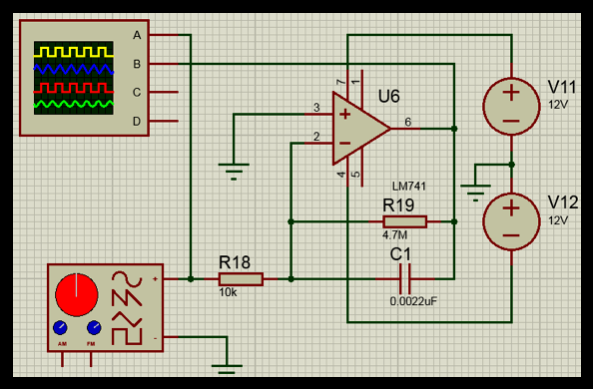
\includegraphics[scale=.315]{s6.png}
\centering \linebreak \linebreak Figure 4.3.0: LM7905 - Fixed negative voltage regulator circuit.
\end{figure}
\begin{center}
\begin{tabular}[.5cm]{ c c }
\toprule
Source Voltage & Voltage in $R_{L}$ \\
\midrule
3.0 V & -2.23 V \\
\cmidrule{1-2}
4.0 V & -3.21 V \\
\cmidrule{1-2}
5.0 V & -4.20 V \\
\cmidrule{1-2}
6.0 V & -5.02 V \\
\cmidrule{1-2}
7.0 V & -5.02 V \\
\cmidrule{1-2}
8.0 V & -5.02 V \\
\cmidrule{1-2}
9.0 V & -5.02 V \\
\cmidrule{1-2}
10.0 V & -5.02 V \\
\cmidrule{1-2}
11.0 V & -5.02 V \\
\cmidrule{1-2}
12.0 V & -5.02 V \\
\cmidrule{1-2}
13.0 V & -5.02 V \\
\cmidrule{1-2}
14.0 V & -5.02 V \\
\cmidrule{1-2}
15.0 V & -5.02 V \\
\cmidrule{1-2}
16.0 V & -5.02 V \\
\bottomrule
\end{tabular}
\end{center} 

\task {\bfseries\itshape Second Circuit, IC used: 7912:}
\begin{figure}[H]
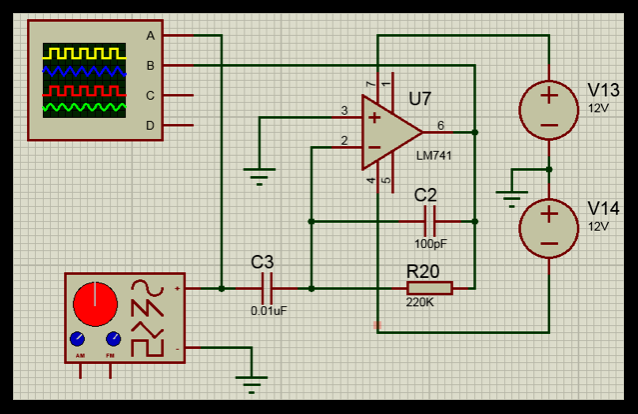
\includegraphics[scale=.3]{s7.png}
\centering \linebreak \linebreak Figure 4.3.1: LM7912 - Fixed negative voltage regulator circuit.
\end{figure}
\begin{center}
\begin{tabular}[.5cm]{ c c }
\toprule
Source Voltage & Voltage in $R_{L}$ \\
\midrule
3.0 V & -2.23 V \\
\cmidrule{1-2}
4.0 V & -3.21 V \\
\cmidrule{1-2}
5.0 V & -4.20 V \\
\cmidrule{1-2}
6.0 V & -5.19 V \\
\cmidrule{1-2}
7.0 V & -6.17 V \\
\cmidrule{1-2}
8.0 V & -7.16 V \\
\cmidrule{1-2}
9.0 V & -8.15 V \\
\cmidrule{1-2}
10.0 V & -9.14 V \\
\cmidrule{1-2}
11.0 V & -10.1 V \\
\cmidrule{1-2}
12.0 V & -11.1 V \\
\cmidrule{1-2}
13.0 V & -12.0 V \\
\cmidrule{1-2}
14.0 V & -12.0 V \\
\cmidrule{1-2}
15.0 V & -12.0 V \\
\cmidrule{1-2}
16.0 V & -12.0 V \\
\bottomrule
\end{tabular}
\end{center} 
\end{tasks}
\end{multicols}

\pagebreak